\documentclass[12pt]{article}
\usepackage{amsmath}
\usepackage{amssymb}
\usepackage{geometry}
\usepackage{enumerate}
\usepackage{natbib}
\usepackage{float}%稳定图片位置
\usepackage{graphicx}%画图
\usepackage[english]{babel}
\usepackage{a4wide}
\usepackage{indentfirst}%缩进
\usepackage{enumerate}%加序号
\usepackage{multirow}%合并行
\title{\large UM-SJTU JOINT INSTITUTE\\Business Basics for Entrepreneurship\\(VX420)\\\ \\\ \\\ \\\ \\\ \\\ \\\ \\\ \\\ \\\ \\\
Individual Report\\\ \\\ Role of Entrepreneurship in Sports Industry \\\ \\\ \\\ \\\ \\\ \\\ \\\ }
\author{Name: Pan Chongdan\\ID: 516370910121}
\date{Date: \today}

\begin{document}
\maketitle
\newpage
\section{Backgrounds of Sports Industry}
Sports has become a big industry whose marketing and commercialization has touched every aspect of our society. Its omnipresent media coverage has increased dramatically over last 10 years. No doubt, sports industry is a social industry affecting many people's life so entrepreneurs have made their forays into sport business and entrepreneurship can play an important role in sport circle. Entrepreneurship can gain much financial return from sports industry because it has become more commercialized and more many are invested in it. More importantly, sports is beneficial to everyone so its social return is enormous. Entrepreneurship in sports industry is quite potential because everyone can be customers.
\section{Development Potential and Executive Summary}
Sport circle is an excellent stage for entrepreneurship. Many kids like football but they seldom have access to it due to geographic restrictions and economic limit. In addition, there are plentiful crazy fans in sports circle but it's hard for them to have a face-to-face chance to communicate with their favourite stars. These are golden opportunities for entrepreneurs to start their business. For entrepreneurs, they can build sports hubs in small areas. The sports hub can include training equipment, sports field and some communication places. Their main customers are targeted as common people living in these areas. Sports clubs can also be customers because the sports hub can help these clubs to find and select talented athletics and enhance clubs' influence. In the future, the sports hub can provide a good environment for fans and residents in small areas to enjoy sports and exercise.  This business's core lies in providing a better condition for poor people to participate in sport, which has a high social value. The sports hub are not necessarily built in small or poor areas because even in some highly-developed areas, it's not always convenient for citizen to participant in any sport they want. Peter Drucker said that entrepreneurship doesn't not require a profit.
\section{Cases Studies and Analysis}
\subsection{Small Company}
For small firms, this business is hard to launch because costs are very high and many large enterprises have already built their own markets in sports industry. Therefore, the best choice for small firms is to cooperate with others or pay more attention to relatively unpopular sports but have a great potential to develop, such as e-sports, an explosively developing sport. Let's take LGD company as an example. In 2008, LGD company is only an unnameable company whose main product is thick chill sauce. However, it invested an undeveloped DotA club and got its naming right. In this cooperation, it improved and built well-operated Internet bars and e-sports hub for e-sports lovers to participate in and be familiar with e-sports, which also help promote e-sports.
\begin{figure}[H]
\centering
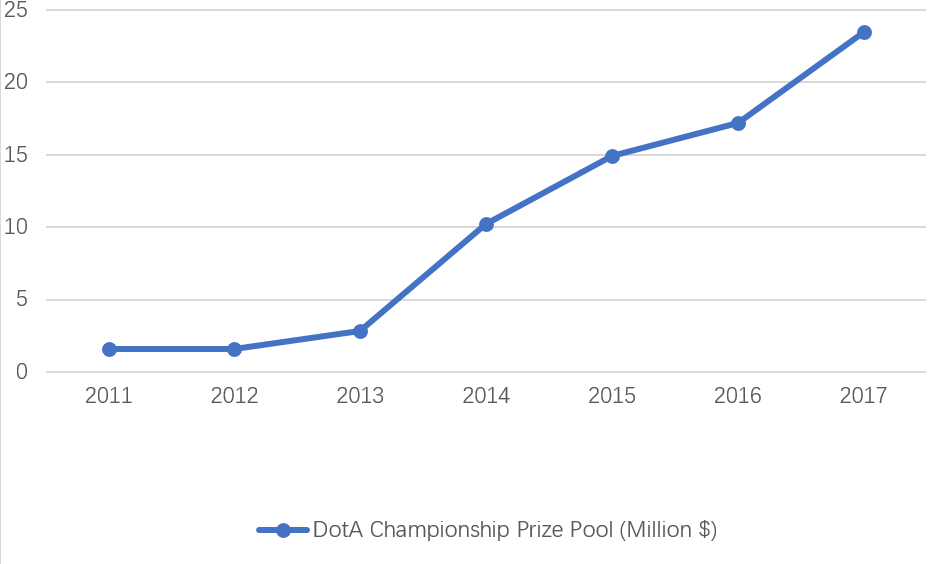
\includegraphics[scale=0.4]{P1.jpg}
\caption{DotA Championship Prize Pool}
\end{figure} 
From Figure 1, we can see that DotA is an e-sport game up-scaling at an astonishing speed. Thanks to the development of DotA and e-sports, LGD company has become widely known to every e-sports lovers and it also has gained massive financial profit from competition prize and operation of Internet hubs. In 2008, e-sport never caught people's eyes, but LGD company played an important role in developing DotA, and its success show that it's such sport that worth investing from small companies.
\subsection{Company of Median Size}
For median companies, the project may be easier to realize since they have deeper pockets and multiple choices. They can cooperate with the government and build pitches for people in poor areas. For instance, a Tai property developer called has managed to shoehorn in several misshapen playing surfaces into the city's densely populated Khlong Toei district. Such business is beneficial to both the company as well as local people because it enables them to play their favourite sports. More importantly, the project enjoys highly social evaluation because it's a public welfare, which will affect the poor people and help the company build a good reputation. 
\begin{figure}[H]
\centering

\includegraphics[scale = 0.6]{P2.jpg}
\caption{Shoehorned pitches in Bangkok}
\end{figure} 
\subsection{Large Enterprise}
For large enterprise like the famous football club Real Madrid, whose membership system ensures its financial support, it can do more to show the entrepreneurship in sports circle. The club often help disaster-affected area to rebuild local sports equipment. Since the club has the most professional sports experts, they can improve the environment for sports lovers. The club has organized many teenager training camp all over the world, which provide golden opportunities for talented teenagers to join the club. It's a win-win project because it also improves the club's players reserves. What's more, it often invites poor fans to club's home court or sends its superstar to condole these fans.
\begin{figure}[H]
\centering

\includegraphics[scale = 0.6]{P3.jpg}
\caption{C. Ronaldo takes a photo with a disabled small fan. }
\end{figure} 
These projects are not aimed to gain profit, but it earns a better reputation and social support for the enterprise. Since the club has a membership system, more social support means more members, which will bring more funds and form a positive circle. As a result, much financial and social returns are gained from the entrepreneurship.
\section{Example of Fitness Industry} 
Nowadays, both single individuals and big companies can operate gyms everywhere, and gym is just like a small sport hub for people around. 
\begin{table}[H]
\centering
\begin{tabular}{|c|c|}
\hline
Year & Revenue income (billion dollars) \\ \hline
1997 & 10                               \\ \hline
2011 & 22                               \\ \hline
2019 & 30                               \\ \hline
\end{tabular}
\caption{Revenue of fitness and recreational sport centres}
\end{table}
According to the study from United States Census Bureau, we can see revenue of fitness and recreational sport centres keeping increasing these years. The result is a highly fragmented industry in which small gyms and entrepreneurs have been able to successfully capture a significant share of the market and to resist the consolidation efforts of larger chains. Fitness entrepreneurs exemplify many of the distinct features attributed to sport entrepreneurs in particular.  
\section{Summary of Development over Last 10 Years}
\begin{figure}[H]
\centering

\includegraphics[scale = 0.3]{P4.jpg}
\caption{The added value and rate of Sports Industry in China }
\end{figure} 
Over last 10 years, Chinese and the world's sports industry has developed dramatically and become much more influential. Although its added rate has become smaller in recent years, sport industry still has a great potential for development and investment and remains a good platform for entrepreneurship. 
\par Currently, many big sports clubs and enterprises have already launched or invested the construction of sports hubs all over the world. Even some individuals like superstars also raise funds to build pitches which have their names. Large entrepreneurship tends to make advertisements or find spokesmen to gain more popularity, then they launch their projects. It is more possible for small entrepreneurship to cooperate with each other, like what they did in fitness industry. They successfully fragment the industry and gain their own profit. Sports industry is still full of opportunities and entrepreneurship will play an increasingly important role in it.
\section{Bibliography}
\begin{enumerate}
\item Hoeber, Larena and Shaw,Sally. Extending sport-based entrepreneurship theory through phenomenological inquiry. \emph{Sports Management Review.}February, 2017.Volume 20, Issue 1, pp92-104.
\item {http://kokofeed.com/2015/10/26/photos-cristiano-ronaldo-puts-a-smile-on-a-disabled-boys-face-with-this-kind-gesture/}
\item http://www.mirror.co.uk/sport/football/news/crazy-misshaped-bangkok-football-pitches-8948481
\item https://en.wikipedia.org/wiki/Entrepreneurship
\item https://en.wikipedia.org/wiki/The\_{International}\_(Dota\_{2})
\end{enumerate}
\end{document}